\documentclass[11pt,a4paper,english]{article}
    \usepackage[latin1]{inputenc}
    \usepackage{amsmath,amsfonts,amssymb}
    \usepackage{enumitem}
    \usepackage{fullpage}
    \usepackage{graphicx}
    \usepackage{tabto}
    \usepackage{etoolbox}
    \usepackage{xcolor}
    \usepackage{hyperref}
    \usepackage{minted}
    \usepackage{parskip}
    \usepackage[title]{appendix}
    \usepackage[font=small,labelfont=bf]{caption}
    \hypersetup{ colorlinks = true}
    \graphicspath{ {./} }

    \title{Bayesian Data Analysis - Assignment 5}
    \author{}

    \begin{document}
        \maketitle
      \definecolor{bg}{rgb}{0.95,0.95,0.95}

      In order to complete this exercise successfully I created a reusable function
      \begin{minted}[bgcolor=bg,fontsize=\small,autogobble]{python}
        generate_chains(sample_size, number_of_chains, burnin_size)
      \end{minted}
      that creates multiple chains with a given sample size and removes the burn-in values.

      To see if the Metropolis algorithm works correctly, I generated \textbf{10 chains} with
      the \textbf{sample size of 3000 each (total: 30000 samples)} and removed the
      \textbf{burn-in size of 500 (total: 5000 samples)}.
      \begin{minted}[bgcolor=bg,fontsize=\small,autogobble]{python}
        chains = generate_chains(
          sample_size=3000,
          number_of_chains=10,
          burnin_size=500
        )
      \end{minted}

      The \textbf{starting points} for each chain are generated randomly. Here is the table of starting points:
      \begin{center}
        \begin{tabular}{l*{6}{c}r}
          $n$ & $\alpha$ & $\beta$ \\
          \hline
          1   &   -2.00   &  7.0  \\
          2   &   3.00    &  23.0 \\
          3   &   2.00    &  18.0 \\
          4   &   4.00    &  16.0 \\
          5   &   1.00    &  26.0 \\
          6   &   2.00    &  24.0 \\
          7   &   -1.00   &  1.0  \\
          8   &   2.00    &  -2.0 \\
          9   &   -1.00   &  14.0 \\
          10  &   1.00    &  20.0 \\
        \end{tabular}
      \end{center}

      The \textbf{proposal/jumping distribution} is calculated using multivariate normal distribution that
      takes the previous $\theta$ value and covariance matrix $cov = \begin{bmatrix}
        0.4 & 1 \\
        1   & 10
      \end{bmatrix}$, which is obtained by deviding the matrix given in the book $\begin{bmatrix}
        4 &  10 \\
        10 & 100
      \end{bmatrix}$ by 10. Here is the python function for jumping distribution:

      \begin{minted}[bgcolor=bg,linenos,fontsize=\small,autogobble]{python}
        def jump(theta_prev, cov):
          j = stats.multivariate_normal(theta_prev, cov)
          theta_sample = j.rvs(1)
          return np.array(theta_sample)
      \end{minted}

      The \textbf{$\widehat{R}$ values} are calculated using theta
      \href{https://github.com/avehtari/BDA_course_Aalto/blob/master/exercises/additional_files/psrf.py}{psrf function}.
      The \textbf{$\widehat{R}$ values} in my case are:

      \begin{center}
        \begin{math}
          \widehat{R}_{\alpha} = 1.00178023 \
          \widehat{R}_{\beta} = 1.00435052
        \end{math}
      \end{center}

      \begin{minted}[bgcolor=bg,linenos,fontsize=\small,autogobble]{python}
        chain = generate_chains(sample_size=10000, number_of_chains=1, burnin_size=500)[0]
        print('Potential Scale Reduction Factor (PSRF) is: ', psrf(chain))
      \end{minted}

      \begin{minted}[bgcolor=bg,fontsize=\small,autogobble]{bash}
        $ Potential Scale Reduction Factor (PSRF) is:  [1.00178023 1.00435052]
      \end{minted}

      The \textbf{interpretation of Rhat values}: if $R$ is not close to 1
      (above 1.1 for example) one may conclude that the tested samples were not
      from the same distribution and that chain might not have been converged yet.
      In my case both $\widehat{R}_{\alpha}$ and $\widehat{R}_{\beta}$ values are
      below $1.1$ which \textbf{means that my generated chains are well converged}.

      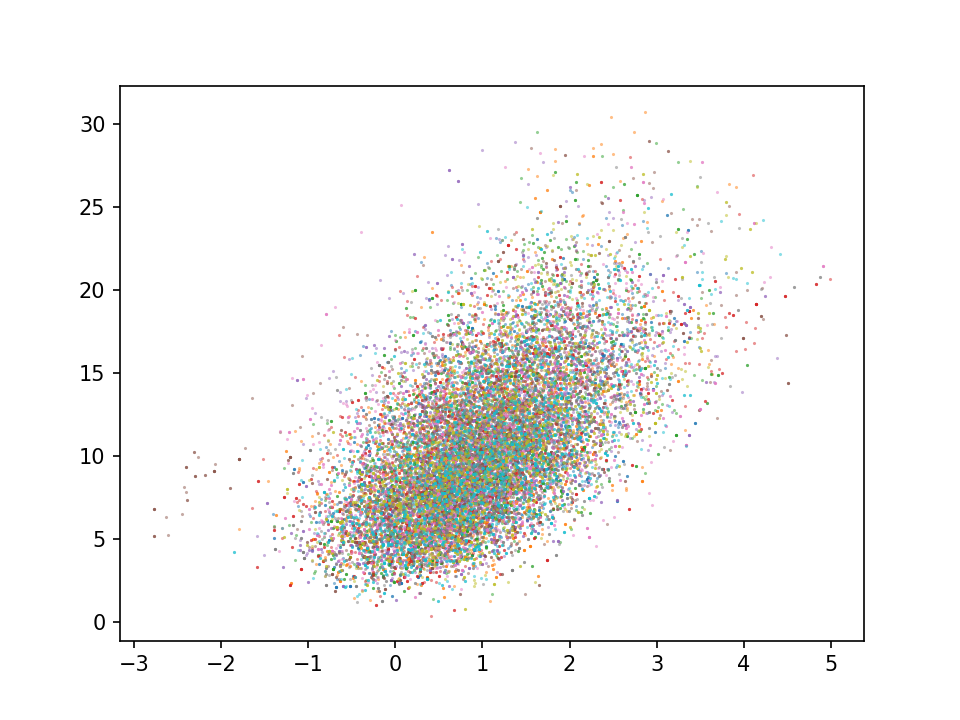
\includegraphics[width=17.7cm]{1_scatter_plot.png}
      \captionof{figure}{A plot of 10 chains with 25000 samples in total.}

      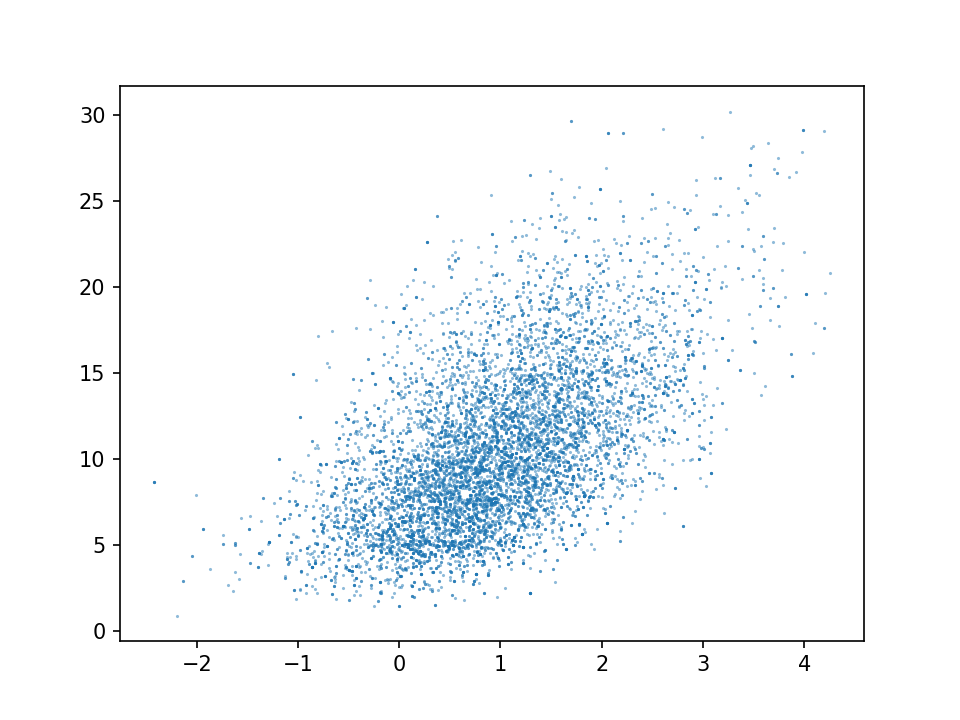
\includegraphics[width=17.7cm]{2_scatter_plot_with_one_chain.png}
      \captionof{figure}{A plot of 1 chain with 10000 samples.}

      \begin{appendices}
        \section{Source code}
        \begin{minted}[bgcolor=bg,linenos,fontsize=\small,autogobble]{python}
          import matplotlib
          matplotlib.use('TkAgg')
          import matplotlib.pyplot as plt
          from scipy import stats
          import numpy as np
          import random
          from psrf import psrf
          from bioarraylp import bioassaylp

          # Init all the params based on the description
          sigma_a = 2
          sigma_b = 10
          mu_a = 0
          mu_b = 10
          cor = 0.5
          cov_matrix = np.array([
              [sigma_a**2,                cor * sigma_a * sigma_b],
              [cor * sigma_a * sigma_b,   sigma_b**2]
          ])
          mean = np.array([mu_a, mu_b])

          doses = np.array([-0.86, -0.3, -0.05, 0.72])
          deaths = np.array([0, 1, 3, 5])
          number_of_animals = np.array([5, 5, 5, 5])

          # reusable functions for Metropolis algorithm
          def jump(theta_prev, cov):
              j = stats.multivariate_normal(theta_prev, cov)
              theta_sample = j.rvs(1)
              return np.array(theta_sample)

          def ratio_can_be_accepted(ratio):
              if ratio >= 1:
                  return True
              else:
                  uniform_random_sample = stats.uniform(0,1).rvs(1)[0]
                  if uniform_random_sample < ratio:
                      return True
                  else:
                      return False

          def get_next_theta(theta_prev, cov):
              theta_new = jump(theta_prev, cov)
              likelihood_theta_new = bioassaylp(
                  theta_new[0],
                  theta_new[1],
                  doses,
                  deaths,
                  number_of_animals
              )
              likelihood_theta_prev = bioassaylp(
                  theta_prev[0],
                  theta_prev[1],
                  doses,
                  deaths,
                  number_of_animals
              )

              prior_multivar_nor = stats.multivariate_normal(mean, cov_matrix)
              prior_new = prior_multivar_nor.pdf(theta_new)
              prior_prev = prior_multivar_nor.pdf(theta_prev)

              post_new = np.exp(likelihood_theta_new) * prior_new
              post_prev = np.exp(likelihood_theta_prev) * prior_prev

              ratio = post_new / post_prev

              if ratio_can_be_accepted(ratio):
                  return theta_new

              return theta_prev

          def trim_burnin(chains, burnin_size):
              trimmed_chains = []
              for chain in chains:
                  trimmed_chains.append(chain[burnin_size:])
              return trimmed_chains

          def generate_chains(sample_size, number_of_chains, burnin_size):
              chains = []
              for i in range(number_of_chains):
                  starting_points = [random.randint(-2, 4), random.randint(-5, 30)]
                  print('starting points', starting_points)
                  chain = [starting_points]

                  for j in range(sample_size):
                      next_theta = get_next_theta(chain[-1], cov_matrix/10)
                      chain.append(next_theta)

                  chains.append(chain)
              return trim_burnin(chains, burnin_size=500)

          chains = generate_chains(sample_size=3000, number_of_chains=10, burnin_size=500)

          for chain in chains:
              plt.plot(
                  np.array(chain)[:, 0],
                  np.array(chain)[:, 1],
                  alpha=0.5,
                  marker='.',
                  linewidth=0,
                  markersize=1,
              )
          plt.savefig('./ex5/report/1_scatter_plot.png', dpi=150)
          plt.figure()

          print('\nSingle chain')
          chain = generate_chains(sample_size=10000, number_of_chains=1, burnin_size=500)[0]
          print('\nPotential Scale Reduction Factor (PSRF) is: ', psrf(chain))
          plt.plot(
              np.array(chain)[:, 0],
              np.array(chain)[:, 1],
              alpha=0.5,
              marker='.',
              linewidth=0,
              markersize=1,
          )
          plt.savefig('./ex5/report/2_scatter_plot_with_one_chain.png', dpi=150)
          plt.figure()


          '''Outputs:
          starting points [-2, 7]
          starting points [3, 23]
          starting points [2, 18]
          starting points [4, 16]
          starting points [1, 26]
          starting points [2, 24]
          starting points [-1, 1]
          starting points [2, -2]
          starting points [-1, 14]
          starting points [1, 20]

          Single chain
          starting points [-1, -5]

          Potential Scale Reduction Factor (PSRF) is:  [1.00178023 1.00435052]
          '''
        \end{minted}
      \end{appendices}
  \end{document}
